
\documentclass[a3paper,landscape,10pt]{article}
\usepackage[a3paper,landscape,margin=1.0cm]{geometry}
\usepackage[T1]{fontenc}
\usepackage{lmodern}
\usepackage{tikz}
\usetikzlibrary{positioning,calc,arrows.meta}
\pagestyle{empty}

\begin{document}
\begin{center}
{\Huge\bfseries StudyFlow}\\[3pt]
{\LARGE Entity Relationship Diagram}\\[3pt]
{\large Core database design for the StudyFlow mobile application}
\end{center}
\vspace{0.15cm}

\begin{center}
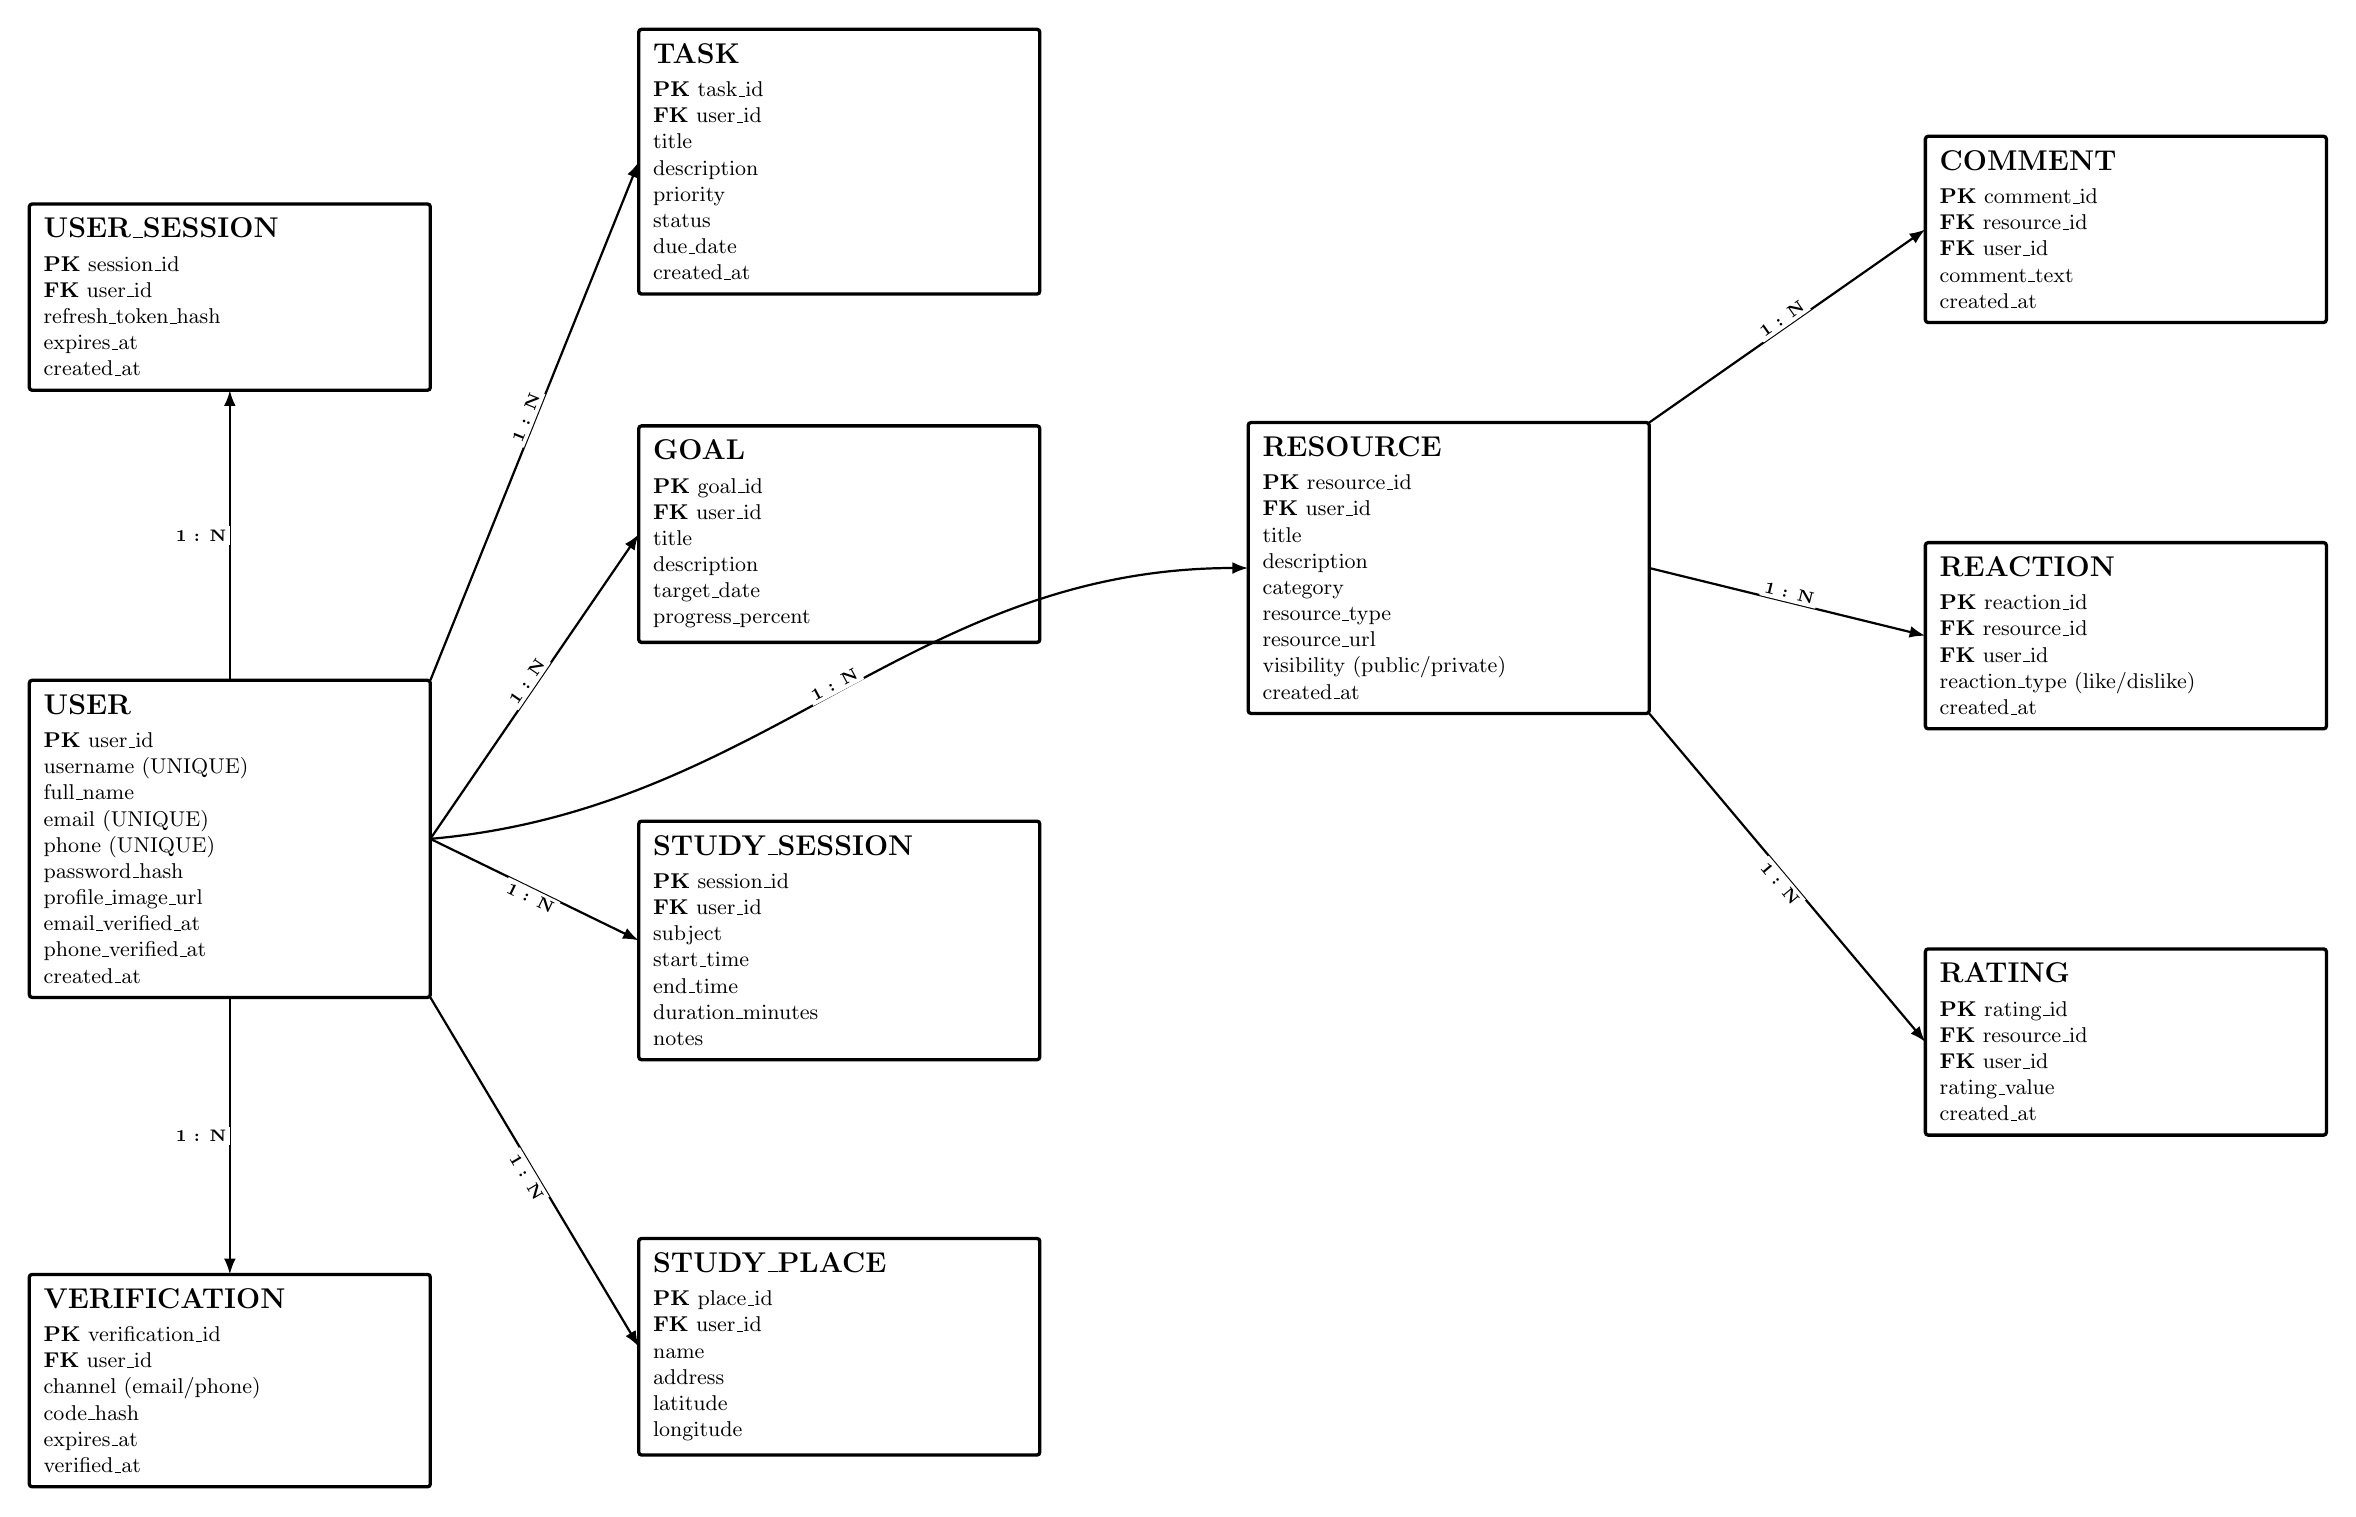
\begin{tikzpicture}[
  scale=0.86, transform shape,
  entity/.style={
    draw=black, very thick, rectangle, rounded corners=1pt,
    fill=white, text width=5.5cm, align=left,
    inner sep=6pt, font=\small
  },
  relation/.style={-{Latex[length=2mm]}, thick},
  card/.style={fill=white, inner sep=1.5pt, font=\bfseries\scriptsize},
  every node/.style={outer sep=0pt}
]
% Authentication and user
\node[entity] (user) at (-11,0) {
  \textbf{\large USER}\\[3pt]
  \textbf{PK} user\_id\\
  username (UNIQUE)\\
  full\_name\\
  email (UNIQUE)\\
  phone (UNIQUE)\\
  password\_hash\\
  profile\_image\_url\\
  email\_verified\_at\\
  phone\_verified\_at\\
  created\_at
};

\node[entity] (usersession) at (-11,8) {
  \textbf{\large USER\_SESSION}\\[3pt]
  \textbf{PK} session\_id\\
  \textbf{FK} user\_id\\
  refresh\_token\_hash\\
  expires\_at\\
  created\_at
};

\node[entity] (verification) at (-11,-8) {
  \textbf{\large VERIFICATION}\\[3pt]
  \textbf{PK} verification\_id\\
  \textbf{FK} user\_id\\
  channel (email/phone)\\
  code\_hash\\
  expires\_at\\
  verified\_at
};

% User-owned planning data
\node[entity] (task) at (-2,10) {
  \textbf{\large TASK}\\[3pt]
  \textbf{PK} task\_id\\
  \textbf{FK} user\_id\\
  title\\
  description\\
  priority\\
  status\\
  due\_date\\
  created\_at
};

\node[entity] (goal) at (-2,4.5) {
  \textbf{\large GOAL}\\[3pt]
  \textbf{PK} goal\_id\\
  \textbf{FK} user\_id\\
  title\\
  description\\
  target\_date\\
  progress\_percent
};

\node[entity] (study) at (-2,-1.5) {
  \textbf{\large STUDY\_SESSION}\\[3pt]
  \textbf{PK} session\_id\\
  \textbf{FK} user\_id\\
  subject\\
  start\_time\\
  end\_time\\
  duration\_minutes\\
  notes
};

\node[entity] (place) at (-2,-7.5) {
  \textbf{\large STUDY\_PLACE}\\[3pt]
  \textbf{PK} place\_id\\
  \textbf{FK} user\_id\\
  name\\
  address\\
  latitude\\
  longitude
};

% Resources and interactions
\node[entity] (resource) at (7,4) {
  \textbf{\large RESOURCE}\\[3pt]
  \textbf{PK} resource\_id\\
  \textbf{FK} user\_id\\
  title\\
  description\\
  category\\
  resource\_type\\
  resource\_url\\
  visibility (public/private)\\
  created\_at
};

\node[entity] (comment) at (17,9) {
  \textbf{\large COMMENT}\\[3pt]
  \textbf{PK} comment\_id\\
  \textbf{FK} resource\_id\\
  \textbf{FK} user\_id\\
  comment\_text\\
  created\_at
};

\node[entity] (reaction) at (17,3) {
  \textbf{\large REACTION}\\[3pt]
  \textbf{PK} reaction\_id\\
  \textbf{FK} resource\_id\\
  \textbf{FK} user\_id\\
  reaction\_type (like/dislike)\\
  created\_at
};

\node[entity] (rating) at (17,-3) {
  \textbf{\large RATING}\\[3pt]
  \textbf{PK} rating\_id\\
  \textbf{FK} resource\_id\\
  \textbf{FK} user\_id\\
  rating\_value\\
  created\_at
};

% User relationships: cardinality labels are placed near the endpoints.
\draw[relation] (user.north east) -- node[card,above,sloped] {1 : N} (task.west);
\draw[relation] (user.east) -- node[card,above,sloped] {1 : N} (goal.west);
\draw[relation] (user.east) -- node[card,below,sloped] {1 : N} (study.west);
\draw[relation] (user.south east) -- node[card,below,sloped] {1 : N} (place.west);

\draw[relation] (user.north) -- node[card,left] {1 : N} (usersession.south);
\draw[relation] (user.south) -- node[card,left] {1 : N} (verification.north);

\draw[relation] (user.east) to[out=5,in=180] node[card,above,sloped] {1 : N} (resource.west);

% Resource relationships
\draw[relation] (resource.north east) -- node[card,above,sloped] {1 : N} (comment.west);
\draw[relation] (resource.east) -- node[card,above,sloped] {1 : N} (reaction.west);
\draw[relation] (resource.south east) -- node[card,below,sloped] {1 : N} (rating.west);

\end{tikzpicture}
\end{center}

\vspace{0.15cm}
\noindent
\fbox{\parbox{0.96\textwidth}{
\textbf{Legend:}\quad PK = Primary Key \qquad FK = Foreign Key \qquad
1:N = One-to-Many Relationship\\[3pt]
\textbf{Design rules:}
Each task, goal, study session, saved study place, and resource belongs to one user.
Resources are public by default but may be marked private. A comment, reaction, or rating
belongs to one resource and one user. Enforce UNIQUE(resource\_id, user\_id) on REACTION
and RATING so each user has at most one current reaction and one rating per resource.
Store password and verification-code hashes, never plaintext secrets. Store uploaded files
in cloud storage; RESOURCE.resource\_url holds the resulting URL or external media link.
}}
\vfill
\begin{center}
{\small\itshape StudyFlow --- CSE 510 Mobile Application Development Lab}
\end{center}
\end{document}
